% This is "sig-alternate.tex" V2.0 May 2012
% This file should be compiled with V2.5 of "sig-alternate.cls" May 2012
%
% This example file demonstrates the use of the 'sig-alternate.cls'
% V2.5 LaTeX2e document class file. It is for those submitting
% articles to ACM Conference Proceedings WHO DO NOT WISH TO
% STRICTLY ADHERE TO THE SIGS (PUBS-BOARD-ENDORSED) STYLE.
% The 'sig-alternate.cls' file will produce a similar-looking,
% albeit, 'tighter' paper resulting in, invariably, fewer pages.
%
% ----------------------------------------------------------------------------------------------------------------
% This .tex file (and associated .cls V2.5) produces:
%       1) The Permission Statement
%       2) The Conference (location) Info information
%       3) The Copyright Line with ACM data
%       4) NO page numbers
%
% as against the acm_proc_article-sp.cls file which
% DOES NOT produce 1) thru' 3) above.
%
% Using 'sig-alternate.cls' you have control, however, from within
% the source .tex file, over both the CopyrightYear
% (defaulted to 200X) and the ACM Copyright Data
% (defaulted to X-XXXXX-XX-X/XX/XX).
% e.g.
% \CopyrightYear{2007} will cause 2007 to appear in the copyright line.
% \crdata{0-12345-67-8/90/12} will cause 0-12345-67-8/90/12 to appear in the copyright line.
%
% ---------------------------------------------------------------------------------------------------------------
% This .tex source is an example which *does* use
% the .bib file (from which the .bbl file % is produced).
% REMEMBER HOWEVER: After having produced the .bbl file,
% and prior to final submission, you *NEED* to 'insert'
% your .bbl file into your source .tex file so as to provide
% ONE 'self-contained' source file.
%
% ================= IF YOU HAVE QUESTIONS =======================
% Questions regarding the SIGS styles, SIGS policies and
% procedures, Conferences etc. should be sent to
% Adrienne Griscti (griscti@acm.org)
%
% Technical questions _only_ to
% Gerald Murray (murray@hq.acm.org)
% ===============================================================
%
% For tracking purposes - this is V2.0 - May 2012
\documentclass{sig-alternate}
\usepackage{algorithm}
\usepackage{algpseudocode}
\usepackage{booktabs}
\usepackage{resizegather}
%%switch case statement
%\newcommand{\SWITCH}[1]{\STATE \textbf{switch} (#1)}
%\newcommand{\ENDSWITCH}{\STATE \textbf{end switch}}
%\newcommand{\CASE}[1]{\STATE \textbf{case} #1\textbf{:} \begin{ALC@g}}
%\newcommand{\ENDCASE}{\end{ALC@g}}
%\newcommand{\CASELINE}[1]{\STATE \textbf{case} #1\textbf{:} }
%\newcommand{\DEFAULT}{\STATE \textbf{default:} \begin{ALC@g}}
%\newcommand{\ENDDEFAULT}{\end{ALC@g}}
%\newcommand{\DEFAULTLINE}[1]{\STATE \textbf{default:} }
%%switch case statement
%\let\footnotesize\scriptsize
%\newsavebox{\supbox}% Superscript box
%\newcommand{\bsup}{\begin{lrbox}{\supbox}$\tt\scriptstyle}% Superscript begin
%\newcommand{\esup}{$\end{lrbox}{}^{\usebox{\supbox}}}% Superscript end
%\def\eg{\latinabbrev{e.g}}
%\def\ie{\latinabbrev{i.e}}
\algnewcommand{\LineComment}[1]{\State \(\triangleright\) #1}
%\renewcommand{\labelenumi}{(\alph{enumi})}
\usepackage{ multirow
,cite
,hyperref
,url
,graphicx
}
\usepackage[numbers]{natbib}     % this is a better citation system
\usepackage{natbib}     % this is a better citation system
\usepackage{expl3}
\usepackage[table]{xcolor}
\usepackage{textgreek}
%\newcommand{\hl}[1]{\textcolor{red}{#1}} % please rephrase
%\usepackage{ifthen}
%\usepackage{amssymb}
%\newboolean{showcomments}
%\setboolean{showcomments}{false}
%\ifthenelse{\boolean{showcomments}}
%{\newcommand{\nbc}[3]{
%{\colorbox{#3}{\bfseries\sffamily\scriptsize\textcolor{white}{#1}}}
%{\textcolor{#3}{\sf\small$\blacktriangleright$\textit{#2}$\blacktriangleleft$}}
%}
%}
%{\newcommand{\nbc}[3]{}
% \renewcommand{\hl}[1]{#1} % please rephrase
%}
%%%Example USE command. Just change the command name as per your name. 
%\newcommand\mukta[1]{\nbc{Mukta}{#1}{blue}}
%\newcommand\roy[1]{\nbc{CR}{#1}{red}}
%\newcommand\mondal[1]{\nbc{MM}{#1}{blue}}
%\renewcommand{\labelitemi}{$\bullet$}
%\usepackage{color}
%\newcommand{\hilight}[1]{\colorbox{yellow}{#1}}
%\newcommand{\hilightnote}[1]{\colorbox{red}{#1}}
\begin{document}
%
% --- Author Metadata here ---
\conferenceinfo{Cascon}{'2015 Toronto, Canada}
%\CopyrightYear{2007} % Allows default copyright year (20XX) to be over-ridden - IF NEED BE.
%\crdata{0-12345-67-8/90/01}  % Allows default copyright data (0-89791-88-6/97/05) to be over-ridden - IF NEED BE.
% --- End of Author Metadata ---
%\title{A Task-Oriented User Study for Evaluating Visualized Extractive Summaries of Bug Reports}
\title{ 
%should we read and analyze bug reports: 
%\hilight
%An Empirical Study - The Effectiveness of Term-Frequency Based (LSI, VSM) and LDA Based Techniques for Locating Bugs in Large Software Project.}
%Terrm-Frequency vs Latent Dirichlet Allocation for Bug Localization in Large  Projects: An Empirical Study
Improved Bug Localization using Keyword-Source Token Co-occurrence.
%An Automatic Query Reformulation Based Bug Localization Technique using Keyword-Source Code Association Relations.
}
%{Should We Read and Analyze Bug Reports:}
%An Interactive Visualization using Extractive Summaries and Topic Evolution\vspace{-.4cm} }
%\title{Interactive Visualisation of Bug Reports using Topic Evolution and Extractive Summaries: Detail Methodologies and A Task-Oriented User Study}
%\title{Alternate {\ttlit ACM} SIG Proceedings Paper in LaTeX
%Format\titlenote{(Produces the permission block, and
%copyright information). For use with
%SIG-ALTERNATE.CLS. Supported by ACM.}}
%\subtitle{[Extended Abstract]
%\titlenote{A full version of this paper is available as
%\textit{Author's Guide to Preparing ACM SIG Proceedings Using
%\LaTeX$2_\epsilon$\ and BibTeX} at
%\texttt{www.acm.org/eaddress.htm}}}
%
% You need the command \numberofauthors to handle the 'placement
% and alignment' of the authors beneath the title.
%
% For aesthetic reasons, we recommend 'three authors at a time'
% i.e. three 'name/affiliation blocks' be placed beneath the title.
%
% NOTE: You are NOT restricted in how many 'rows' of
% "name/affiliations" may appear. We just ask that you restrict
% the number of 'columns' to three.
%
% Because of the available 'opening page real-estate'
% we ask you to refrain from putting more than six authors
% (two rows with three columns) beneath the article title.
% More than six makes the first-page appear very cluttered indeed.
%
% Use the \alignauthor commands to handle the names
% and affiliations for an 'aesthetic maximum' of six authors.
% Add names, affiliations, addresses for
% the seventh etc. author(s) as the argument for the
% \additionalauthors command.
% These 'additional authors' will be output/set for you
% without further effort on your part as the last section in
% the body of your article BEFORE References or any Appendices.
\numberofauthors{1} %  in this sample file, there are a *total*
% of EIGHT authors. SIX appear on the 'first-page' (for formatting
% reasons) and the remaining two appear in the \additionalauthors section.
%
\author{
% You can go ahead and credit any number of authors here,
% e.g. one 'row of three' or two rows (consisting of one row of three
% and a second row of one, two or three).
%
% The command \alignauthor (no curly braces needed) should
% precede each author name, affiliation/snail-mail address and
% e-mail address. Additionally, tag each line of
% affiliation/address with \affaddr, and tag the
% e-mail address with \email.
%
% 1st. author
%\alignauthor
%Ben Trovato\titlenote{Dr.~Trovato insisted his name be first.}\\
%       \affaddr{Institute for Clarity in Documentation}\\
%       \affaddr{1932 Wallamaloo Lane}\\
%       \affaddr{Wallamaloo, New Zealand}\\
%       \email{trovato@corporation.com}
%% 2nd. author
%\alignauthor
%G.K.M. Tobin\titlenote{The secretary disavows
%any knowledge of this author's actions.}\\
%       \affaddr{Institute for Clarity in Documentation}\\
%       \affaddr{P.O. Box 1212}\\
%       \affaddr{Dublin, Ohio 43017-6221}\\
%       \email{webmaster@marysville-ohio.com}
%% 3rd. author
%\alignauthor Lars Th{\o}rv{\"a}ld\titlenote{This author is the
%one who did all the really hard work.}\\
%       \affaddr{The Th{\o}rv{\"a}ld Group}\\
%       \affaddr{1 Th{\o}rv{\"a}ld Circle}\\
%       \affaddr{Hekla, Iceland}\\
%       \email{larst@affiliation.org}
%\and  % use '\and' if you need 'another row' of author names
% 4th. author
\alignauthor Shamima Yeasmin~~~Mohammad Masudur Rahman~~~Chanchal K. Roy~~~ Kevin A. Schneider\\
       \affaddr{Department of Computer Science, University of Saskatchewan, Canada}\\
       %\affaddr{University of Saskatchewan}\\
       %\affaddr{Canada}\\
       \email{shy942@mail.usask.ca, \{chanchal.roy, kevin.schneider\}@usask.ca}
%% 5th. author
%\alignauthor Sean Fogarty\\
%       \affaddr{NASA Ames Research Center}\\
%       \affaddr{Moffett Field}\\
%       \affaddr{California 94035}\\
%       \email{fogartys@amesres.org}
%% 6th. author
%\alignauthor Charles Palmer\\
%       \affaddr{Palmer Research Laboratories}\\
%       \affaddr{8600 Datapoint Drive}\\
%       \affaddr{San Antonio, Texas 78229}\\
%       \email{cpalmer@prl.com}
}
% There's nothing stopping you putting the seventh, eighth, etc.
% author on the opening page (as the 'third row') but we ask,
% for aesthetic reasons that you place these 'additional authors'
% in the \additional authors block, viz.
\additionalauthors{Additional authors: John Smith (The Th{\o}rv{\"a}ld Group,
email: {\texttt{jsmith@affiliation.org}}) and Julius P.~Kumquat
(The Kumquat Consortium, email: {\texttt{jpkumquat@consortium.net}}).}
\date{30 July 1999}
% Just remember to make sure that the TOTAL number of authors
% is the number that will appear on the first page PLUS the
% number that will appear in the \additionalauthors section.

\maketitle
\begin{abstract}
Bug localization is one of the most challending tasks undertaken by the developers during software maintenance.
Existing studies mostly rely on lexical similarity between the bug reports and source code for bug localization.
However, such similarity always does not exist, and these studies suffer from vocabulary mismatch issues.
In this paper, we propose a bug localization technique that (1) not only uses lexical similarity between bug report and source code documents  
but also (2) exploits the co-occurrences between keywords from the past reports and source tokens from corresponding changed code.
Experiments using a collection of ~6000 bug reports show that our technique performs significantly higher in terms of Hit@K and MAP
than one state-of-the-art IR-based bug localization techniques using TF-IDF and other LDA based technique.
%Bug localization is the process of locating the source codes that need to be changed in order to fix a given bug. It is a challenging as well as time-consuming task for a large and evolving software project as the project team could receive large number of bug reports. For locating a given bug the developer must search through a large number of files in a project, which is not a trivial task.
%Bug localization is a software maintenance task in which a developer formulates a query from information presented in a bug report and using this query to search through the software system in order to determine the portion of the source code that needs to be changed or modified for fixing that given bug. 
%However, existing approaches for locating buggy files are of either static or dynamic bug localization technique. Static localization technique mainly focus on source code of a software system where dynamic technique consider execution traces of the system. 
%Existing studies on bug localization suffer from two issues - one is vocabulary miss-match from bug reports to their relevant source location and the other is computing with large scale search space.
%Most of the existing studies are based on lexical similarity that often produce low accuracy results.
%Because, there is a significant difference between the natural language texts used in bug reports and code tokens in source codes.
%In order to reduce the issue with lexical similarty, an association can be established between bug reports and fixed source code files.
%one is low accuracy in performance measure and the other is small-scale experiments. 
%The success of existing studies depended much on the quality of the queries as a poorly designed query is prone to retrieve irrelevant documents. However, designing a query is challenging as it requires certain level of knowledge and expertise of the developer regarding the code base.
%So in this paper, we are proposing a bug localization technique utilizing association maps between keywords extracted from previously fixed bug reports and fixed source code files. 
%Our proposed approach is also narrowing down the search space i.e., number of source code files need to be inspect every time.
%Our proposed approach also automatically suggest helpful reformulation of a given query based on semantic similarity between terms.
%In this paper, we are proposing a bug localization approach, which consists of two parts- (1) query processing and (2) localization of newly reported bug.  First, our proposed approach automatically suggest helpful reformulation of a given query based on semantic similarity between terms.
%Here, initial query is collected from the content of a newly reported bug’s title and description. 
%Our proposed approach mines all fixed bugs for a given project and its source code repository and retrieve candidate terms based on word co-occurrence measure. 
%The idea is to consider the semantic similarity between terms. 
%Finally, our proposed approach suggests the helpful reformulation of a given query iteratively.
%Second, we are proposing a bug localization technique utilizing association maps between keywords extracted from previously fixed bug reports and fixed source code files. 
%We will construct association maps by using information collected from fixed bug reports, commit logs and source code repository. 
%Here, the idea is to exploit keyword-source code relationship for recommending a list of candidate source code files that need to be fixed. 
%We will collect tokens from bug report title and description. 
%We know that source code files which are fixed can be found from commit logs. 
%So, using these two types of information we can construct maps between token and source code files. 
%These association maps are used to recommend source code files for a newly reported bug report.
%We perform a large-scale experiments on 6000 bug reports and 12000 source code files.
%We compare the performance of our proposed approach
%In this paper, we work 
%with two information retrieval based static bug localization techniques:  TF-IDF based and  LDA based. 
%Results suggest that our proposed approach significantly outperforms existing techniques.
%We work with several datasets and compare the performance of both bug localization techniques.

%\hilight{highly}
%significantly 
%rated
% as well as accepted 
%than 
%the non-visualized summary for quick comprehension of bug reports.
%Prior to the assignment of a newly reported bug to an appropriate developer, the triager
%%(i.e.,
%(e.g.,
%manager) attempts to categorize it into existing categories and 
%looks for duplicate bugs.
%The goal is to reuse existing knowledge to fix or resolve the new bug, and she often spends
%a lot of time in reading a number of bug reports. 
%During the fixation or resolution of a bug, 
%When fixing or resolving a bug,
%a developer also consults with a series of relevant bug reports from the repository
%in order to maximize the knowledge required for the fixation.
%It is also preferable that developers new to a project first familiarize themselves with the project along with the reported bugs before actually working 
%on it.
%which is likely to help her avoid or resolve the similar reported issues. 
%Manually analyzing a large collection of bug reports
%not much effective, and it costs a significant amount of efforts and time. 
%is time-consuming and ineffective, and
%To address this challenge, 
%Because of the sheer 
%%weight of 
%numbers and 
%%the 
%size of the bug reports, manually analyzing a collection of bug reports is time-consuming and ineffective. One of the ways to mitigate the problem is to analyze summaries of the bug reports instead of analyzing full bug reports, and there have been a number of summarization techniques proposed in the literature. Most of these techniques generate extractive summaries of bug reports.
%However, an extractive summary is often created by choosing a certain number of statements from the bug report.
%The statements are extracted out of their contexts, and thus often lose their consistency, which makes it hard for a manager or a developer to comprehend the reported bug from the extractive summary. In order to assist the managers as well as the developers, in our previous ERA paper, we thus proposed an interactive visualization for the bug reports that visualizes not only the extractive summaries but also the topic evolution of the bug reports.  
%In our previous work, we proposed a prototype that offers useful insights derived from a collection of bug reports as well as provides a visualization for the extractive summary of a bug report.
%In our previous ERA paper, we proposed a 
%prototype
%that assists developers review a project's bug reports by interactively visualizing insightful information regarding the bug reports using topic analysis. 
%In addition, in order to reduce developers' time and efforts when studying a bug report, the proposed prototype also provides an extractive summary visualization of each bug report. 
%In this paper, we describe the methologies we have used for both visualization. 
%In this paper, we provide a detail description of the methodologies we have used in our previously proposed prototype. We also conduct a task-oriented user study in order to validate the effectiveness of the previously proposed extractive summary visualization. The results from the user study indicate that the performance of bug report visualized summary is highly rated as well as accepted than the non-visualized summary during the comprehension of bug report quickly.
%In this paper, we extend our previously proposed ptototype by evaluating the affectiveness of extractive summary visualization technique with a task-oriented user study. The results from the user study indicate that the performance of bug report visualized summary is highly rated as well as accepted than the non-visualized summary during the comprehension of bug report quickly. We also provide a detail description of the methodologies we have used in our previously proposed visualizations.
% related to extracitive summay and topic evolution of bug reports.
%and highly accepted by the user.
%One of the ways to mitigate the problem is to analyze summaries of the bug reports instead of analyzing full bug reports, and there have been a number of summarization techniques proposed in the literature. 
%This paper provides a sample of a \LaTeX\ document which conforms,
%somewhat loosely, to the formatting guidelines for
%ACM SIG Proceedings. It is an {\em alternate} style which produces
%a {\em tighter-looking} paper and was designed in response to
%concerns expressed, by authors, over page-budgets.
%It complements the document \textit{Author's (Alternate) Guide to
%Preparing ACM SIG Proceedings Using \LaTeX$2_\epsilon$\ and Bib\TeX}.
%This source file has been written with the intention of being
%compiled under \LaTeX$2_\epsilon$\ and BibTeX.
%The developers have tried to include every imaginable sort
%of ``bells and whistles", such as a subtitle, footnotes on
%title, subtitle and authors, as well as in the text, and
%every optional component (e.g. Acknowledgments, Additional
%Authors, Appendices), not to mention examples of
%equations, theorems, tables and figures.
%To make best use of this sample document, run it through \LaTeX\
%and BibTeX, and compare this source code with the printed
%output produced by the dvi file. A compiled PDF version
%is available on the web page to help you with the
%`look and feel'.
\end{abstract}

% A category with the (minimum) three required fields
\category{H.4}{Information Systems Applications}{Miscellaneous}
%A category including the fourth, optional field follows...
\category{D.2.8}{Software Engineering}{Metrics}[complexity measures, performance measures]

%\terms{Theory}

\keywords{Bug Report, Topic Evolution, Summary, Visualization}
\section{Introduction}\label{sec:introduction}
%Bug localization is a software maintenance task in which a developer formulates a query using information in a bug report and using this query to search through the software system in order to determine the portion of the source code that needs to be changed or modified for fixing that given bug. 
Checking
Bug localization is the process of locating the source codes that need to be changed in order to fix a given bug. 
Locating buggy files is time-consuming and costly if it is done by manual effort, especially for the large software system when the number of bug of that system becomes large. Therefore, effecting methods for locating bugs automatically from bug reports are highly desirable. 
In automatic bug localization technique, it takes a subject system as an input and produces a list of entities such as classes, methods etc. against a search query. For example, information retrieval based techniques rank the list of entities by predicted relevance and return a ranked list of entities or source codes which may contain the bug. 
The bug localization techniques are also affected by the fact of designing effective query. If a query contains inadequate information, then the retrieval results will not be relevant at all. One other thing that the performance of existing bug localization approach did not reach to an accepted level and so far those studies showed good results for a small set of bugs. Therefore,
%However, static bug localization technique has an advantage over dynamic technique, as it does not require any working subject system rather it can apply on any stage of a system. 
in this paper, we apply a bug localization technique on large dataset that exploits an association link established from bug report repository to source code base through commit logs. 
%We also process the query in a reformulation manner so that the semantic importance between terms both in bug reports and code base could be utilized.

%In this paper, we replicate some major bug localization techniques \cite{Jian} \cite{Anh} \cite{Saha} \cite{Moreno} \cite{Lukins}, and then perform a comparison of their performance on large-scale data. 
In existing studies, information retrieval techniques  \cite{Jian} \cite{Saha} \cite{Moreno} \cite{Anh} \cite{Lukins} are applied to automatically search for relevant files based on bug reports.
In one case of Text Retrieval (TR) based approaches, \citet{Jian} propose BugLocator using revised Vector Space Model (rVSM), which requires the information extracted from bug reports and source codes. One of the issue association with TR-based technique is treating source codes as flat text that lacks structure. But exploiting source code structure can be a useful way to improve bug localization accuracy.
Due to the fuzzy nature of information retrieval, textually matching bug reports against source
files may have to concede noise (less relevant but accidentally matched words). However, large files are more
likely to contain noise as usually only a small part
of a large file is relevant to the bug report. So, by treating
files as single units or favoring large files, the techniques are more
likely to be affected by the noise in large files. So, \citet{Saha} present BLUiR, which retrieve structural information from code constructs.
However, bug reports often contain stack-trace information, which may provide direct clues for possible faulty files. Most existing approaches directly treat the bug descriptions as plain texts and do not explicitly consider stack-trace information. Here, \citet{Moreno} combine both stack trace similarity and textual similarity to retrieve potential code elements. 
To deal with two issues associated with source code structure and stack trace information, 
\citet{Chu}  proposed  a technique that use segmentation i.e., divides each source code file into segments and use stack-trace analysis, which significantly improve the performance of BugLocator.
LDA topic-based approaches \cite{Anh} \cite{Lukins} assume that the textual contents of a bug report and it's corresponding buggy source files share some technical aspects of the system.
Therefore, they develop topic model that represents those technical aspects as topic. 
However, existing bug localization approaches applied on small-scale data for evaluation so far.
Besides the problem of small-scale evaluations, the performance of the existing bug localization methods can be further improved too. For example, using Latent Dirichlet Allocation (LDA), only buggy files for 22\% of Eclipse 3.1 bug reports are ranked in the top 10 [25]. 
But, now it is an important research question to know how effective these approaches are for locating bugs in large-scale (i.e., big data).
 In the field of query processing
\citet{Sisman}  proposed a method that examines the files retrieved for the initial query supplied by a user and then selects from these files only those additional terms that are in close proximity to the terms in the initial query. Their \cite{Sisman} experimental evaluation on two large software projects using more than 4,000 queries showed that the proposed approach leads to significant improvements for bug localization and outperforms the well-known QR methods
in the literature.
There are two common issues associated with existing studies. First, 
most of the bug localization techniques exploit lexical similarity measure for retrieving relevant files from the code base. So, it is expected that the search query constricted from new bug report should contain keywords similar to code constructs in code base. This issue demands developers or users  previous expertise on the given project, which can not be guaranteed in real world. 
Second, closely related to the first issue there is another well known problem called vocabulary mismatch. In order to convey the same concept on both search query (i.e., new bug report) and source code files the developers tend to use different vocabularies. This issue questions the applicability of exploiting lexical similarity measure.

So, in order to resolve these two issues, in our work we propose a bug localization approach that combines lexical similaority with word co-occurrence measue. 
Our proposed technique exploits the association of keywords extracted from fixed bug report with their changed source code location. Here, the main idea is to capture information from a collection of bug reports and exploit them for locating relevant source code location.
 So our approach not (1) only relies on the lexical similarity measure between big reports and source code files for bug localization, and (2) but also addresses the vocabulary mismatch problem by using a keyword-source map constructed from fixed bug information.
%In the field of bug localization several works have been done such as Text Retrieval based approaches  \cite{Jian} \cite{Saha} \cite{Moreno}, LDA topic-based approaches \cite{Anh} \cite{Lukins} and so on.
%In the case of Text Retrieval based approaches, \citet{Jian} propose BugLocator using revised Vector Space Model (rVSM),  \citet{Saha} present BLUiR, which retrieve structural information from code constructs,  \citet{Moreno} combine both stack trace similarity and textual similarity to retrieve potential code elements.  
%The former two approaches \cite{Jian} \cite{Anh} require the information extracted from bug reports and source codes, where the later approach \cite{Anh} considers stack trace information in addition those two software artifacts. 
%On the other hand, LDA topic-based approaches  \cite{Anh} \cite{Lukins} assume that the textual contents of a bug report and it's corresponding buggy source files share some technical aspects of the system.
%Therefore, they develop topic model that represents those technical aspects as topic. However, both approaches applied on small-scale data for evaluation so far. But, now it is an important research question to know how effective these approaches are for locating bugs in large-scale (i.e., big data).

We also replicate two state of the art bug localization techniques in order to compare the performance of our proposed approach with these two.
%So, in this project, we will replicate some existing bug localization techniques and apply them on large-scale software project for bug localization.
% Here, the research goals are (i) perform a comparison among several bug localization techniques for large-scale software projects from several perspective such as performance, effectiveness etc., (ii) we will also try to discover the drawbacks of deploying them on large scale, and (iii) finally we would like to propose a technique that can work better for large-scale bug localization.

%\citet{Wang}  intregates a bug prediction technique used in Google which analyzes version history, with a bug localization technique BugLocator \cite{Jian}, which analyzes similar bug reports of a given bug report, and  the state-of-the-art bug localization technique BLUiR \cite{Saha} which considers code structures. This technique is named as Amalgam \cite{Wang}, which achieves significant improvement in terms of Mean Average Precision (MAP) when compared to BugLocator and BLUiR. 


%Typically, existing IR-based approaches treat each source file as a single unit, and 
%due to the fuzzy nature of information retrieval, textually matching bug reports against source
%files may have to concede noise (less relevant but accidentally matched words). Large files are more
%likely to contain noise as usually only a small part
%of a large file is relevant to the bug report. By treating
%files as single units or favoring large files, we are more
%likely to be affected by the noise in large files. 
%On the other hand, Bug reports often contain stack-trace information, which may provide direct clues for possible faulty files. Most existing approaches directly treat the bug descriptions as plain texts and do not explicitly consider stack-trace information. 
%So deal with these two issues, 
%\citet{Chu}  proposed  a technique that use segmentation i.e., divides each source code file into segments and use stack-trace analysis, which significantly improve the performance of BugLocator.
 
%Most of the existing IR-Based bug localization techniques have a limitation that they are evaluted by the projects written in Object Oriented Programming Languages, particularly Java. In order to investigate the effectiveness of those techniques for other widely used language C 
%\citet{Saha2} created a benchmark dataset consisting of more the 7500 bug reports and evaluate BLUiR bug localization tool using this dataset and they found that IR-based bug localization in C software at the file level is overall as effective as in Java software.

%Code clone is a  code analysis technique that iinvolves locating duplicated sections of code in software
%projects.
%\citet{Beard} examined the application of code clone location techniques in the context of bug localization and found code clone localization appears to be an ideal technique for automated bug localization.
%\citet{Chatterji}
%performed a study involving 43 graduate students that investigates the usefulness of code clone information for
%performing a bug localization task. The results of this study showed that participants who first identified a defect then used it to look for clones of the defect were more effective than participants who used the clone information before finding any defects.

%The vector space model (VSM) with the standard tf-idf weighting scheme (VSMnatural), has been shown to outperform
%nine other state-of-the-art IR techniques. However, there are multiple VSM variants with different weighting schemes, and
%their relative performance differs for different software systems.
%Based on this observation, \citet{Shaowei} proposed to compose various VSM variants, modelling their composition as an optimization problem.
%\citet{Shaowei} demonstrated that theirr approach can achieve better
%performance than VSM with the standard tf-idf weighting
%scheme (VSMnatural ).

%In the field of query processing
%\citet{Sisman}  proposed a method that examines the files retrieved for the initial query supplied by a user and then selects from these files only those additional terms that are in close proximity to the terms in the initial query. Their \cite{Sisman} experimental evaluation on two large software projects using more than 4,000 queries showed that the proposed approach leads to significant improvements for bug localization and outperforms the well-known QR methods
%in the literature.

\section{An Example Use Case Scenario}\label{sec:usecase}
Note:
Provide an example such as say for bug B1 source code files F1, F2, F3 are modified or changed. Now a new bug B has similar to B1 in terms of cosine similarity. Then prove that F1, F2, F3 or one or two of them are contained in the list of files which would be changed or modified for fixing that new bug B.
Lets consider a bug having ID "" from Eclipse-UI-Platform software. From Git repository it is discoverd that so far n number of file have been modified in order to fix this bug. We also csn find the source code address of those changed files. Now, 

In another example, show that the words or keywords of a bug B are aslo presented in the source code files F1, F2 or F3. 
\section{Existing Approaches}\label{sec:existing}
We have replicated two existing bug localization approaches: (i) TF-IDF based bug localization approach and (ii) LDA topic based bug localization technique. In the following subsections we will briefly discuss each of them.
\subsection{TF-IDF Based Bug Localization Technique:}
In this technique, each source code file is ranked based on source code file scores and similar bugs information. Source code file contains words those can be also occurred in the bug reports. This is considered as a hint to locate buggy files. If a new bug is similar to a given previously located bug, then there is a possibility that the source code files located for the past bug can provide useful information in finding buggy files for that new bug. Based on these two assumptions, we compute scores for all source code files for a given project. However, we need to focus on some concepts which are required to understand the  system. They are described as follows:


%\subsection{
\textbf{Ranking based on TF-IDF calculation:}
The basic idea of a TF-IDF model is that the weight of a term in a document is increasing with its occurrence frequency in this specific document and decreasing with its occurrence frequency in other documents \cite{Jian}.
In this approach we have used a revised Vector Space Model (rVSM) proposed by \citet{Jian} in order to index and rank source code files. 
The main difference between classic VSM and revised VSM is that in case of revised version logarithm variant is used in computing term frequency. The equation is:
\begin{equation}
tf(t+d)=log(f_{td})+1
\end{equation}
Here \textit{tf} is the term frequency of each unique term \textit{t} in a document \textit{d} and \textit{f\textsubscript{td}} is the number of times term \textit{t} appears in document \textit{d}.
So the new equation of revised VSM model is as follows:

%\begin{equation*}
%rVSMScore(q,d)=g(\#term)\times cos(q,d)
%\end{equation*}

%\begin{equation}
\begin{multline}\label{rVSMequation}
	rVSMScore(q,d)=g(\#term)\times cos(q,d)
	\\
	\frac{1}{1+e^{-N(\#terms))}}\times \frac{1}{\sqrt{\sum_{t\epsilon q}}((logf_{tq}+1)\times log(\frac{\#docs}{n_{t}}))^{^{2}}}\times 
	\\
	\frac{1}{\sqrt{\sum_{t\epsilon d}((log {f_{td}+1})\times log(\frac{\#docs}{n_{t}}))^{2}}}\times
	\\
	\sum_{t\epsilon q\bigcap d}(logf_{tq}+1)\times (logf_{td}+1)\times log(\frac{\#docs}{n_{t}})^{2}
\end{multline}
%\end{equation}
This \textit{rVSM} score is calculated for each query bug report \textit{q} against every document \textit{d} in the corpus. However, in the above equation \textit{\#terms} refers to the total number of terms in a corpus, \textit{n\textsubscript{t}} is the number of documents where term \textit{t} occurs.

%\subsection{
\textbf{Ranking based on similar bug information}
\begin{figure}
	\centering
	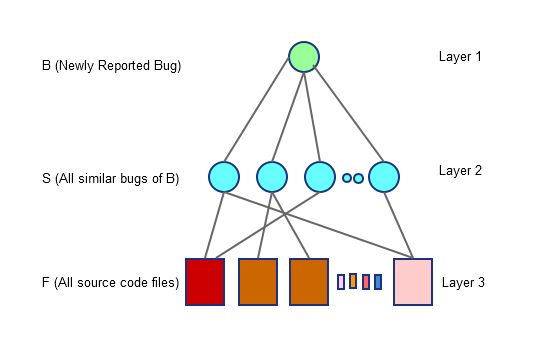
\includegraphics[scale=0.65]{3layers}
	\caption{Bug and its Similar Bug Relationship with Source Code Files:}
	\label{fig:BSBR}
\end{figure}
The assumption of this ranking is similar bugs of a given bug tend to modify similar source code files. Here, we construct a 3-layer architecture as described in \cite{Jian}. In the top layer (layer 1) there is a bug \textit{B} which represents a newly reported bug. All previously fixed bug reports which have non-negative similarity with bug  \textit{B} are presented in second layer. In third layer all source code files are shown. In order to resolve each bug in second layer some files in the corpus were modified or changed, which are indicated by a link between layer 2 and layer 3. Foe all source code files in layer 3, similarity score is computed, which can be referred to as degree of similarity. The score can be defined as:

\begin{equation}\label{Simiequation}
SimiScore=\sum_{All S_{i} that connect to F_{j}}(Similarity(B,S_{i})/n_{i})
\end{equation} 
Here, similarity between newly reported bug \textit{B} and previously fixed bug \textit{S\textsubscript{i}} is calculated based on cosine similarity measure and \textit{n\textsubscript{i}} is the total number of link \textit{S\textsubscript{i}} has with source code files in layer 3.

%\subsection
\textbf{Combining Both Ranks:}
We combine the both scores based on source code score and similar bugs score as in \cite{Jian} as follows:
\begin{equation}
FinalScore=(1-\alpha )\times N(rVSMScore)+\alpha \times N(SimiScore)
\end{equation}
%Here, \textit{\textalpha} is a weighting function and the value of \textit{\textalpha} is in between 0 and 1. In our experiment we use 0.2 as the value of \textit{\textalpha}
\subsection{LDA Topic Based Bug Localization Technique:}
The main assumption behind this technique is the textual content of the bug reports and their associated buggy source code files tend to describe some common technical aspects. So, if  we could identify the technical topics extracted from both bug reports and source codes, we could recommend the files shared technical topics with the newly reported bug reports. If a newly reported bug has similar technical topics with some previously fixed bug reports, the fixed files could be a good candidate files for newly reported bug.

LDA (Latent Dirichlet Allocation) is a probabilistic and fully generative topic model. It is used to extract latent (i.e., hidden) topics, which are presented in a collection of documents. It also model each document as a finite mixture over the set of topics [add link here]. In LDA, similarity between a document \textit{d} and a query \textit{q} is computed as the conditional probability of the query given that document \cite{Lukins2}.

\begin{equation}
Sim(q,d_{i})=P(q|d_{i})=\prod_{q_{k}\epsilon q}P(q_{k}|d_{i})
\end{equation}

Here \textit{q\textsubscript{k}} is the \textit{k}th word in the query {q} Thus, a document (i.e., source code file) is relevant to a query if it has a high probability of generating the words in the query.

We perform the following steps in order to localize buggy files for newly reported bug using LDA based approach:


\begin{itemize}
	\itemsep 0em
	\item Apply topic modeling on the source code files. The output contains a certain number of topics and some associated keywords for each topic. We also get some other distribution files such as document-topic, word-topic etc.
	\item Now work with the documents topic distribution file. Make a list of source code documents or files for each topic. So, we wiill have a list that contain all topics and their associated source code documents.
	\item Here our query is the newly reported bug. This contains information in the bug reports such as title and short description etc. We all do inference for this query using a topic modeling tool. It will extract all topic associated with the query (i.e., newly reported bug).
	\item Now we need to work with topic keywords. We are going to perform a comparison between newly reported bug or the given query and source code files using topic information. That means we will compare topic-keywords associated with topics inferred for the query with topic-keywords of each topic extracted from source code documents.
	\item We will rank them based on topic-keyword similarity. So, now we know which are the top most topics, and we already have information regarding topic-document relationship, we will retrieve all source code files associated with all those top most topic as recommended buggy files.
	%\item A detailed description of methodologies for visualizing topic evolution extracted from bug reports.
	%\item A detailed description of methodologies for visualizing bug report extractive summaries.
	%\item Evaluation of visualized bug report extractive summary by conducting a task-oriented user study.
\end{itemize}
\section{Proposed System Diagram}\label{sec:proposedsystemDiagram}
Our proposed approach combine lexical similarity and co-occurence similarity measure.  \citet{Jian} proposed BugLocator based on two different similarity scores- one is rVSM score and the other one is Simi score. In our porposed bug localization approach, we retrieve relevant ranked files based on three different scores- 1) rVSM, 2) Simi and 3) Word Co-occurence. So,
we have divided our approach into two different sections or parts- 1) calculate rVSM and Simi scores and co-occurence measure and 2) combine all three scores in order to localize recommended buggy source files for a given newly reported bug. As we have combined two existing scores with our proposed word co-occirence score, we will discuss the system diagram of association map database in Part I and then we represent our overall system diagram in Part II.
%\subsection{Part I: Query Reformulation}
%\begin{figure*}
%\centering
%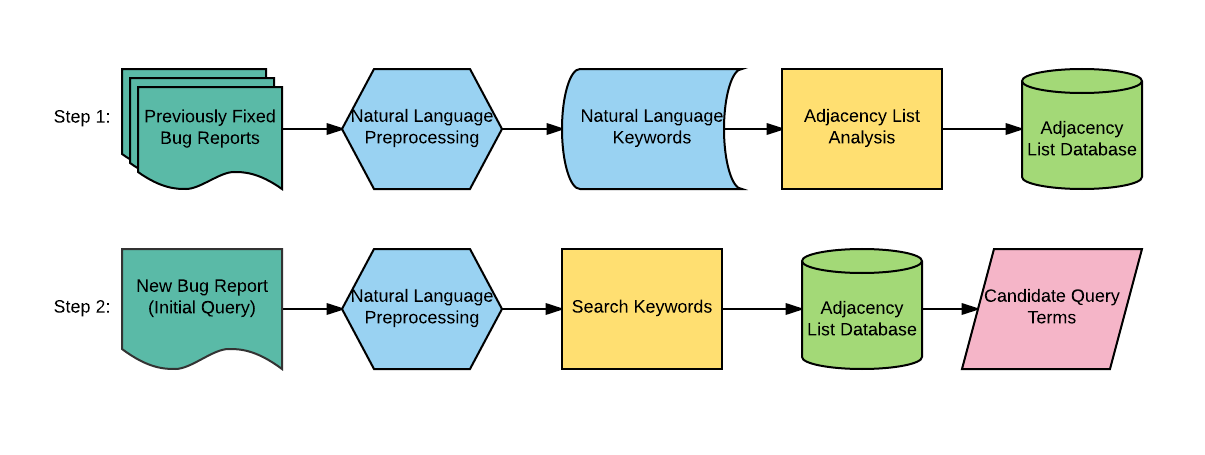
\includegraphics[scale=0.75]{QueryReformulation}
%\caption{Proposed System Diagram: Query Reformulation}
%\label{fig:QR}
%\end{figure*}
%
%In this part, we reformulate the initial query, where a newly reported bug report is considered as an initial query. The system diagram for this part is given in Fig. \ref{fig:QR}.
%Here, this part is also divided into two separate sections. First one is creating adjacency list database and the later one is reformulating the initial query by exploiting the adjacency list database.
%
%In the first section, we create adjacency list database for bug reports collection. 
%A typical bug report contains several pieces of information such as title, description of the reported issue and developers comments and so on. At first we create a corpus containing information collected from title, description and developers comments of each bug report. Then we preprocess the collected information. For preprocessing we first remove stop words from the corpus and then perform stemming on words. We know that a collection of bug reports contains a large number of keywords or words. 
%So after preprocess the corpus we retrieve a large collection of natural language keywords. 
%Then, we construct adjacency list database that contains semantically similar keywords for each of these unique keywords.
%Word co occurrence is often considered as a proxy for semantic relevance between words in natural language  texts. So, we construct a database containing adjacent keyword list for each of the individual keywords collected from the title, description  and developers comments of the bug reports collection. 
%
%We know, a newly reported bug report contains title and description of the reported issue what we call the initial query for the retrieval system. In the second section, we collect this initial query from the user or developer and preprocess them by removing stop words and perform stemming on it. Now this preprocessed query consists of collection of natural language keywords. 
%We use these keywords to
%leverage the information contained in the adjacency list database in order to suggest keywords for reformulating the initial query. Here the idea is, for each natural keywords presented in the preprocessed initial query, we retrieve the adjacent keywords list from the adjacency database. We use cosine similarity metric to measure the similarity between the adjacent keywords list of each query term and other individual terms presented in the adjacency list database. Using this formula we formulate candidate keywords for the initial query, which we mention as candidate query terms.
 
\subsection{Part I: Mapping Bug Source Code Links}
In Part I, we construct an association map database - between keywords extracted from previously fixed bug reports collection and source code links. The system diagram for Part I is given in Fig. \ref{fig:MP}.

This mapping construction involves two steps.
At first we create association map using information contained in bug reports collection and commit logs. We collect information from title and description fields of each bug report. There are also developers comment section in a bug report, which is highly informative. But large documents also tend to reduce performance by taking too long to process. So, we reluctant to include developers comments of each bug report. However, we extract keywords from each bug report after preprocessing them such as stop word removal. 
%In this part, information are collected from bug report, version repository and source code repository. 
In version repository, we have commit logs, where the developers commit for several changes in a software project. For example, when a bug report is fixed, the developer who fixed this bug also creates a commit log containing which type of change he had to made to resolve the bug associated with the location of the source code files where the change has made. So, if we analyze commit logs, we can retrieve source code files information which have been changed in order to fix a given bug. Here the idea is, we first extract keywords from bug report and source code links for the same bug from commit log and then construct an association map database containing this mapping information. The links between keywords and source code links can be described as: each or several keywords can be linked to one or more source code links and each source code link can be linked to one or several keywords. This way we connect keywords and source code links to form an association map database named keyword-source code links. 

%Then we analyze commit logs and source code repository. We collect source code links for a solved bug from the commit log and each of these source code contains source code contents. We preprocess these source code content by removing stop words from them but we do not perform stemming on them. Then we connect each source code links to one or may be more source code tokens to form our another association map database named source code-code token links.
\begin{figure}
\centering
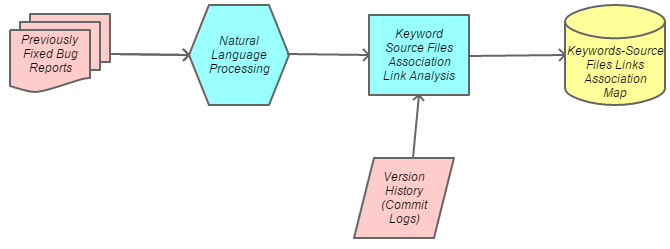
\includegraphics[scale=0.55]{Map}
\caption{Proposed System Diagram: Mapping}
\label{fig:MP}
\end{figure}


\begin{figure*}
	\centering
	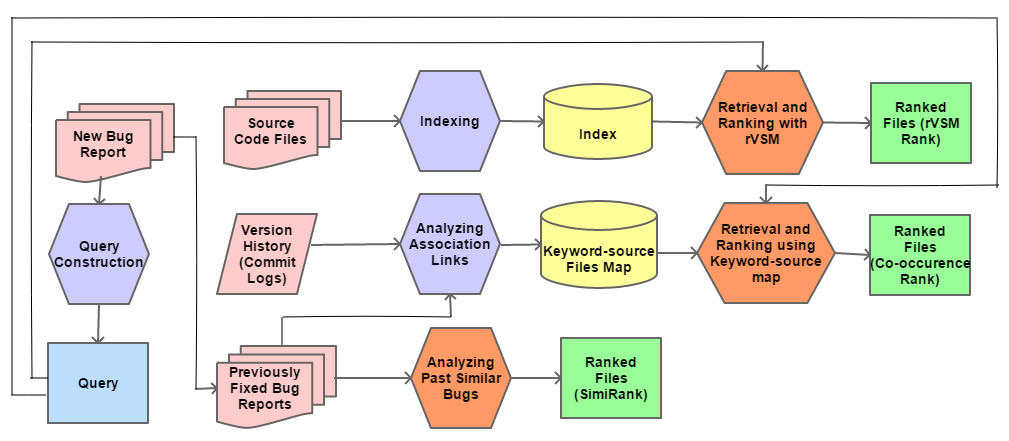
\includegraphics[scale=0.75]{SD1}
	\caption{Proposed System Diagram: Bug Localization}
	\label{fig:BL}
\end{figure*}

\subsection{Part II: Bug Localization Using rVSM, and Co-occurence Ranks}

The system diagram for this part has illustrated in Fig. \ref{fig:BL}.
In our system, we have three different ranks i.e., rVSM, Simi and Co-occurence. We utlize an existing technique proposed by \citet{Jian} for computing rVSM and Similarity scores. Basically, rVSM is a TF-IDF based score, which is measured between query and source code files.
On the other hand, Simi score refers to that fact that if a bug is similar to another bug, then they both tend to relate to same sources. However, we describe both scores in Section \ref{sec:existing}.
We have constructed an association map databases from keywords collected from bug report to its source code location information in Section \ref{sec:proposedsystemDiagram}.
For the candidate keyword tokens for the initial query, we exploit association map database (i.e., keyword-source code links) and retrieve the relevant source code files. We use some heuristic functions in order to combine three ranks and recommend buggy relevant source files.  
%and this is one part of our predicted locations for buggy source code files.

% these source code files we also find some keywords extracted from those source code files.  

\section{Proposed Approach}\label{sec:proposedApproach}
Our proposed approach consists of two parts - (i) constructing association map databases and (ii) retrieve relevant buggy source code files. 
%\subsection{Part I: Query Reformulation}
%In this part, we reformulate the initial query provided by the developer. We form the initial query from the title and description sections of a newly reported bug. However, this part is further divided into two sections - (i) Construction of Adjacency List Database and (ii) Reformulation of an Initial query. Both of them are described belows:
%%In this part, we reformulate the query provided to the system in the form of new bug report. We include the content extracted from \textit{Title} and \textit{Description} fields of the bug report.
%\begin{algorithm}[!t]
%\caption{Query Reformulation}
%\label{algo}
%\begin{algorithmic}[1]
%\Procedure{QUERY}{$Q$}\Comment{$Q$: initial search query}
%\State $Q' \gets$ \{\}\Comment{reformulated search query}
%\LineComment{collecting keywords from the initial search query}
%\State $K \gets$ collectKeywords($Q$)
%\LineComment{collecting candidate terms}
%%\For{Keyword $K_i \in$ $K$}
%\State $T_b \gets$ getCandidateTermsFromBugReportsRepos($K$)
%%\EndFor
%%\For{Keyword $K_i, K_j$ $\in$ $K$}
%%\State $T_{so} \gets$ getCandidateTermsFromSourceCodeRepos($K$)
%%\EndFor
%\LineComment{estimating semantic similarity of the candidates}
%\For{Candidate $T_i$ $\in$ $T_b$}
%\State $Adj_{T_i} \gets$ getAdjacencyListFromDB($T_i$)
%\For{Keyword $K_j \in K$}
%\State $Adj_{K_j} \gets$ getAdjacencyListFromDB($K_j$)
%\LineComment{contextual similarity between words}
%\State $S_{cos} \gets$ getCosineSimilarity($Adj_{T_i}, Adj_{K_j}$) 
%\State $R_b[T_i].score \gets R_b[T_i].score + S_{cos}$
%\EndFor
%\EndFor
%%\For{Candidate $T_i$ $\in$ $T_{so}$}
%%\For{Keyword $K_j \in K$}
%%\LineComment{co-occurrence between words}
%%\State $S_{cof} \gets$ getCo-occurrenceFreq($T_i, K_j $) 
%%\State $R_{so}[T_i].score \gets R_{so}[T_i].score + S_{cof}$
%%\EndFor
%%\EndFor
%\LineComment{ranking and selection of candidates}
%\State $SR_b \gets$ sortCandidates($R_b$)
%%\State $SR_{so} \gets$ sortCandidates($R_{so}$)
%\State $SR_{Top_b} \gets$ selectTopK($SR_b$)
%%\State $SR_{Top_{so}} \gets$ selectTopK($SR_{so}$)
%\LineComment{collecting semantically similar/relevant terms}
%\State $R \gets$ $SR_{Top_p}$ 
%\LineComment{reformulate the initial query}
%\State $Q' \gets$ reformulate($Q, R$)
%\State \textbf{return} $Q'$
%\EndProcedure
%\end{algorithmic}
%\end{algorithm}
%%\vspace{-.4cm}
%\setlength{\textfloatsep}{2pt}
%
%\textbf{Construction of Adjacency Database:} We create adjacent list database for both previously fixed bug reports collection and source code files. In the adjacent list database we have keywords or terms, where each term is associated with other 20 terms based on their co-occurrence property in the entire corpus.
%
%\textbf{Query Reformulation:} 
%Proposed algorithm for this section is provided in Algorithm \ref{algo}.
%Our initial search query contains the content collected from title and description of a newly reported bug report.
%We then preprocess them by removing stop words and perform stemming on it. This preprocessed query consists of collection of keywords \textit{K}.
%We retrieve the candidate terms from the adjacent list database of bug reports. Here, candidate terms are unique keywords presented in the adjacency list database. We then estimate the semantic similarity of the candidate terms with each keyword of the preprocessed query term. 
%For each term from the adjacent list database, we retrieve the adjacency list of that term. Then we compare the adjacency list of each term with the adjacency list of each query keyword. Here, we use cosine similarity measure for computing similarity between two adjacent lists. This process is done in Algorithm \ref{algo} from line 8 to 16. 
%We calculate score based on cosine similarity scores. 
%Then we rank the candidate terms and select top n candidate terms in order to reformulate the initial query. 
%Our original query is now replaced by those top ranked candidate keywords.
\subsection{Construction of Association Map Database Between Bug Reports and Source Files}
In this part, we construct two association map databases - one is between keywords and source code links extracted from bug reports and commit messages respectively and other one is between source code links and code token extracted from commit messages and source code content respectively. This section can be further divided into several parts: keyword extraction from bug reports, source code link extraction from commit logs, keyword- source code linking, code tokens extraction from source codes and source code-code token linking. They are discussed in the followings:

\begin{algorithm}[!t]
\caption{Construction of Association Map Database Between Bug Reports and Source Files}
\label{map}
\begin{algorithmic}[1]
\Procedure{BUG REPORTS }{$BRC$}\Comment{$BRC$: a collection of bug reports}
\State $MAP_{KS} \gets$ \{\}\Comment{an association map}
\LineComment{creating adjacency map database from the bug reports collection}
\State $MAP_{adj} \gets$ createAdjacencyDatabase($BRC$)
\LineComment{creating a map that links keywords into their bug ids}
\State $MAP_{kb} \gets$ createKeywordsToBugMaps($MAP_{adj}$)
\LineComment{collecting unique keywords from keywords to bug map}

%\LineComment{preprocess the collected keywords}
%\For{Keyword $K_i \in$ $K$}
\State $KB \gets$ collectKeywords($MAP_{kb}$)

\LineComment{Linking keywords from a bug report into its change set files}
\For{keywords $KB_{_i}$ $\in$ $KB$}
\State $BUG_{id} \gets$ retrieveBugIds ($K_i$)
\For{each bug id $BUG_{id_j} \in BUG_{id}$}
\State $SF_{links} \gets$ getLinkedSourceFiles($BUG_{id}$)
\LineComment{maps all source code files to its keywords}
%\State $MAO_{BUG_{id}} \gets$ linkSourceCodeFiles$Adj_{T_i}, Adj_{K_j}$) 
\State $MAP[KB_i].links \gets MAP[KB_{i}].links + SF_{links}$
\EndFor
\EndFor

\LineComment{collecting all keyword-source files links}
\State $MAP_{KS} \gets$ $MAP[KB]$ 
%\LineComment{put them into map}
%\State $MAP \gets$ mapping()
\State \textbf{return} $MAP_{KS}$
\EndProcedure
\end{algorithmic}
\end{algorithm}



\textbf{Keyword Extraction from Bug Reports:} We collect title, description and developers comments from each fixed bug report in a collection of bug reports. We perform standard natural language pre-processing on the corpus such as stop word removal, splitting and stemming. The purpose of removing stop words is that they contain very little semantic for a sentence. The process of stemming step extracts the root of each of the word. We use this stop word list [link] during stop word removal and this stemmer [link]for stemming. 

\textbf{Source Code Link Extraction from Commit Logs:}
We go through all commit messages and try to find those commit message that contain keywords related to bug fix such as fix, fixed and so on. Each of these commit messages presents other information such as the ID of bug report for which it was created and the links of the changed source code files. We then construct a relationship against each fixed bug report ID into their changed source code files links.

\textbf{Keyword- Source Code Linking:}
At this point, in one side we have pre-processed keywords associated with each bug report and on the other side we have a relationship information between bug report ID and buggy source code links. We construct a bipartite graph between keywords collected from a bug report to its buggy source code locations. Here, one or more keywords can be linked to one or more buggy source code files links and a source code file link can be linked to one or more keywords.

\textbf{Calculating Co-occurence Scores}
A query typically contains several keywords or words. For each keyword, we look for relevant source files in the keyword-source files association map. We assume these files are relevant because we created the map between the content of bug reports and their buggy source files. However, when we analysis these links for all keywords in a query, a relevant file can be found more than once. So we normalize the frequency of source files using standard TFIDF normalization technique. Then we recommend first Top-K files with their CoOccScores. The equation for computing co-occurence score is given belows:
\begin{equation}\label{CoOccequation}
SimiScore=\sum_{All S_{i} that connect to W_{j}}(Link(W{j},S_{i}))
\end{equation}
Here, the links between keyword and source file is 1 if they are connected in the association map and 0 otherwise.
%\begin{algorithm}[!t]
%\caption{Construction of Association Map Database Between Source Files and Code Tokens}
%\label{mapsfandct}
%\begin{algorithmic}[1]
%\Procedure{SOURCE FILES }{$SF$}\Comment{$SF$: a collection of source code files}
%\State $MAP_{FT} \gets$ \{\}\Comment{an association map}
%\LineComment{creating adjacency map database from source code files to its code tokens}
%\State $SF_{all} \gets$ getAllSourceCodeFiles($SF$)
%
%
%\LineComment{Linking files from a project corpus into its code tokens}
%\For{Source Files $SF_{_i}$ $\in$ $SF_{all}$}
%\State $CD_{i} \gets$ retrieveCodeTokens ($SF_i$)
%%\For{each bug id $BUG_{id_j} \in BUG_{id}$}
%\State $CD_{pi} \gets$ preprocessSourceCodeTokens($CD_{i}$)
%\LineComment{generate a link between source files to its preprocessed code contents}
%%\State $MAO_{BUG_{id}} \gets$ linkSourceCodeFiles$Adj_{T_i}, Adj_{K_j}$) 
%\State $MAP[SF_i].tokens \gets MAP[SF_{i}].tokens + CD_{pi}$
%%\EndFor
%\EndFor
%
%\LineComment{collecting all source files-token links}
%\State $MAP_{FT} \gets$ collect ($MAP[KB]$ )
%%\LineComment{put them into map}
%%\State $MAP \gets$ mapping()
%\State \textbf{return} $MAP_{FT}$
%\EndProcedure
%\end{algorithmic}
%\end{algorithm}

  




\begin{algorithm}[!t]
\caption{Recommendation of Buggy Source Code Files}
\label{localization}
\begin{algorithmic}[1]
\Procedure{REFORMULATED QUERY }{$Q'$}\Comment{$Q'$: a reformulated query}
\State $RESULT \gets$ \{\}\Comment{recommended source files}
\LineComment{retrieving source files from keyword-source file map}
\State $SF_{Q'} \gets$ getAllSourceCodeFilesForQuery($MAP_{KS}$)


%\LineComment{Linking files from a project corpus into its code tokens}
\For{Source Files $SF_{Q'_i}$ $\in$ $SF_{Q'}$}
\State $K_{i} \gets$ retrieveKeywordsForSourcFile ($MAP_{KS}$)
%\For{each bug id $BUG_{id_j} \in BUG_{id}$}
\State $K_{Q'_i} \gets$ getKeywordsFromReformulatedQuery($Q'$)
\LineComment{contextual similarity between keywords}
%\State $MAO_{BUG_{id}} \gets$ linkSourceCodeFiles$Adj_{T_i}, Adj_{K_j}$) 
%\State $S_cos.\gets getCosineSimilarity($K_{i} ,$K_{Q'_i})
\State $S_{cos} \gets$ getCosineSimilarity($K_{i}, K_{Q'_i}$) 
\State $R_{SF_Q'} \gets$ $S_{cos}$

%\EndFor
\EndFor
\LineComment{ranking and selection of candidates}
\State $SR_Q' \gets$ sortCandidates($R_{SF}$)
%\State $SR_{so} \gets$ sortCandidates($R_{so}$)
\State $SR_{Top_Q'} \gets$ selectTopK($SR_Q'$)
%\State $SR_{Top_{so}} \gets$ selectTopK($SR_{so}$)
\LineComment{collecting top k result}
\State $RESULT \gets$ $SR_{Top_Q'}$ 
%\LineComment{reformulate the initial query}
%\State $Q' \gets$ reformulate($Q, R$)
\State \textbf{return} $RESULT$
%\LineComment{collecting all source files-token links}
%\State $MAP \gets$ collect ($MAP[KB]$ )
%\LineComment{put them into map}
%\State $MAP \gets$ mapping()
%\State \textbf{return} $MAP$
\EndProcedure
\end{algorithmic}
\end{algorithm}

\subsection{Localizing Buggy Source Code Files} 
In this part, we combine existing two approaches with our proposed keyword-source co-occurence relations. One is with rVSM and Simi ranks which are presented in BugLocator and other one is Vector Space Model based technique. So, there are two sub parts of this section.

\textbf{Combination of rVSM, Simi Rank and Co-occurence Rank:}
For each query, we compute the rVSM score against all source codes in the database using equation \ref{rVSMequation} and we also calculate Simi score using equation \ref{Simiequation}. Then we calculate co-occurence scores for the query using equation \ref{CoOccequation}.
We finally combine the three ranks and for that we use a weighting factor \textit{alpha}.
The final equation is given in equation \ref{equationBLme}.
\begin{multline}\label{equationBLme}
	FinalScoreApproach1=(1-\alpha )\times N(rVSMScore)+
	\\ \alpha \times N(SimiScore) + \alpha \times N(CoOccScore)
\end{multline}
We work with different values of \textit{alpha}, which are pre presented in the experiment section.

\textbf{Combinition of VSM and Co-occurence Rank:}
We compute VSM score using Appache Lucene library. Then we combine that score with our CoOccScore using equation \ref{equationVSMme}.
\begin{multline}\label{equationVSMme}
	FinalScoreApproach2=(1-\alpha )\times N(VSMScore)+ \\
	\alpha \times N(CoOccScore)
\end{multline}



\section{Experiment and Discussion}
.

\begin{table}[!t]
%% increase table row spacing, adjust to taste
% if using array.sty, it might be a good idea to tweak the value of
% \extrarowheight as needed to properly center the text within the cells
\caption{Description of Data Sets}
\label{tab:DDSl}
\centering
\scalebox{0.9}{%
%% Some packages, such as MDW tools, offer better commands for making tables
%% than the plain LaTeX2e tabular which is used here.
\begin{tabular}{|c|l|l|}

%\textbf{Month} & $\overline{\textbf{CRD}}$ \\

\hline
\textbf{Project Name}  &  \textbf{\#Source Codes} & \textbf{\#Bug Reports}\\
\hline
{Eclipse Platform Ant} & {6085} & 11732\\
\hline
%\multirow{ 2}{*}{2} & \multirow{ 2}{*}{Editor Outline} & editor xml view outlin content\\
%&& action elem open docum associ\\

\end{tabular}}
\end{table}
\begin{table}[]
	\centering
	\caption{Performance of Bugloactor and proposed technique (rVSM+Simi+Co-Occerence)}
	\label{tab:Performance1}
	\resizebox{3.2in}{!}{%
	\begin{tabular}{@{}|c|c|c|c|c|c|c|@{}}
		\toprule
		%\begin{tabular}[c]{@{}c@{}}\#Bugs for \\ developing \\ map databases\end{tabular} &
		\begin{tabular}[c]{@{}c@{}}\# Test  \\ Case \\ \end{tabular} & \begin{tabular}[c]{@{}c@{}}Bug\\Localization \\ Technique\end{tabular} & \begin{tabular}[c]{@{}c@{}}Top 1\\ \%\end{tabular} & 
		\begin{tabular}[c]{@{}c@{}}Top 5\\ \%\end{tabular} & 
		\begin{tabular}[c]{@{}c@{}}Top 10\\ \%\end{tabular} &
		\begin{tabular}[c]{@{}c@{}} MRR \end{tabular} & 
		\begin{tabular}[c]{@{}c@{}} MAP \end{tabular} \\
		 \midrule
		\multirow{2}{*}{1}  &BugLocator     &  8.89& 24.55&34.32& 0.23 & 0.28 \\  
		& rVSM+Simi+ Co-Score                                                                                                                                               & 14.50                                               & 34.91                                            & 45.86                                                &   0.33  & 0.41    \\ \midrule
		\multirow{2}{*}{2}  &BugLocator     &  9.9& 24.62&34.53& 0.24 & 0.29 \\ 
		& rVSM+Simi+ Co-Score                                                                      & 12.62                                               & 39.04                                              & 49.85                                             &   0.37  &   0.42  \\ \midrule
		\multirow{2}{*}{3}  &BugLocator     &  7.50& 21.32&30.63& 0.21 & 0.24 \\ 
		& rVSM+Simi+ Co-Score                                                                     & 12.01                                            & 33.93                                            & 48.35                                             &   0.34  &  0.38   \\ \midrule
		\multirow{2}{*}{4}  &BugLocator     &  8.1& 21.02&29.13& 0.20 & 0.24 \\ 
		& rVSM+Simi+ Co-Score                                                                    & 15.02                       & 33.63                       & 48.65                                               &  0.33   &  0.42  \\ \midrule 
		\multirow{2}{*}{5}  &BugLocator     &  9.6& 30.63&42.94& 0.29 & 0.32 \\ 
		& rVSM+Simi+ Co-Score                                                                    & 17.71                                                 & 43.84                                                & 56.45                                                  &  0.41   & 0.50     \\ \midrule
		\multirow{2}{*}{6}  &BugLocator     &  10.21& 31.53&43.54& 0.30 & 0.33 \\ 
		& rVSM+Simi+ Co-Score
		&22.22 &
		48.65 &
		58.86 & 0.45 &
		0.58     \\  \midrule
		\multirow{2}{*}{7}  &BugLocator     &  9.61& 30.33&40.84& 0.28 & 0.31 \\ 
		& rVSM+Simi+ Co-Score
		&18.62 &
		47.15 &
		59.76 & 0.44 &
		0.53     \\  \midrule
		\multirow{2}{*}{8}  &BugLocator     &  8.4& 26.13&39.94& 0.26 & 0.28 \\ 
		& rVSM+Simi+ Co-Score
		&18.92 &
		46.55 &
		60.36 & 0.44 &
		0.53    \\  \midrule
		\multirow{2}{*}{9}  &BugLocator     &  11.11& 28.83&40.24& 0.27 & 0.32 \\ 
		& rVSM+Simi+ Co-Score
		&19.82 &
		42.94 &
		56.16 & 0.40 &
		0.52    \\  \midrule
		\multirow{2}{*}{10}  &BugLocator     &  6.6& 20.72&27.93& 0.19 & 0.21 \\ 
		& rVSM+Simi+ Co-Score
		&9.91 &
		33.33 &
		45.65 & 0.31 &
		0.33    \\  \midrule
		\multirow{2}{*}{Average}       &BugLocator     &  8.99\%& 25.87\%&36.40\%& 0.25 & 0.28  \\ 
		& rVSM+Simi+ Co-Score                                                                                                                         & 16.13\%                                                 & 40.40\%                                                 & 52.94\%                                                  &   0.38  &  0.46    \\ \bottomrule
		
	\end{tabular}}
\end{table}


\subsection{Data Collection}
We work with Eclipse data set. We downloaed a git based Eclipse project from git repository \cite{eclipseGit}. We work with Eclipse Platform UI project. Currently it contains 6085 number of Java source codes. These source codes are contained in our source code repository. On the other hand, currently Eclipse Platform UI project contains more than 10K number of bugs where we only work with the bugs which are fixed. We create quires from each bugs considering their title and short summary.
%We have two parts in our corpus. One is source code files downloaded as git based project and another part is bug reports collection. 
All bug reports are collected from \textit{Bugzilla}. In order to obtain the links between previously fixed bugs and source code files, we analyze git project commit message. We ran through all commit messages and track Bug IDs associated with examined source code files.

\subsection{Cross Validation}
We divide our query data into k number of sets. Typically k is 10, but we work with k =5 and k=10. Each set contains a training set and tesing set. Training data is used to create mapping between keywords extracted from bug reports and source code files. 10-fold-cross validation data is presented in table and table.



\begin{table}[]
	\centering
	\caption{Performance of proposed technique (VSM+Co-Occerence) Ranks}
	\label{tab:T3}
	\resizebox{2.7in}{!}{%
		\begin{tabular}{@{}|c|c|c|c|c|c|c|@{}}
			\toprule
			%\begin{tabular}[c]{@{}c@{}}\#Bugs for \\ developing \\ map databases\end{tabular} &
			\begin{tabular}[c]{@{}c@{}}\# Test  \\ Case \\ \end{tabular} & \begin{tabular}[c]{@{}c@{}}\#Bugs for \\ locating \\ issues\end{tabular} & \begin{tabular}[c]{@{}c@{}}Top 1\\ \%\end{tabular} & \begin{tabular}[c]{@{}c@{}}Top 5\\ \%\end{tabular} & \begin{tabular}[c]{@{}c@{}}Top 10\\ \%\end{tabular} & MRR & MAP \\ \midrule
			\multirow{2}{*}{1}& VSM & 23.28& 45.50&55.82& 0.43 & 0.60 \\ 
			& VSM + Co-Score & 25.98                                               & 48.82                                            & 58.27                                                &   0.47  & 0.66 \\ \midrule
			
			\multirow{2}{*}{2}                                                                               & VSM & 22.81 & 45.09 & 54.91 & 0.43 & 0.60 \\   &VSM + Co-Score                                                                     & 26.53                                               & 48.81                                              & 58.89                                             &   0.47  &   0.67  \\ \midrule
			\multirow{2}{*}{3}                                                                               & VSM & 19.95 & 39.63 & 50.27 & 0.39 & 0.52 \\   &VSM + Co-Score                                                                       & 21.22                                            & 46.42                                            & 56.76                                             &   0.44  &  0.57   \\ \midrule
			\multirow{2}{*}{4}                                                                               & VSM & 21.22 & 42.97 & 52.52 & 0.42 & 0.57 \\   &VSM + Co-Score                                                                      & 21.75                       & 46.68                       & 58.35                                                &  0.44   &  0.59  \\ \midrule 
			\multirow{2}{*}{5}                                                                               & VSM & 26.79 & 51.72 & 61.80 & 0.49 & 0.67 \\   &VSM + Co-Score                                                                       & 29.18                                                 & 53.31                                                 & 60.74                                                  &  0.50   & 0.72     \\ \midrule
			\multirow{2}{*}{6}                                                                               & VSM & 23.47 & 49.33 & 60.27 & 0.46 & 0.62 \\   &VSM + Co-Score 
			&24.93 &
			51.72 &
			62.07 & 0.49 &
			0.67     \\  \midrule
			\multirow{2}{*}{7}                                                                               & VSM & 28.45 & 52.13 & 62.77 & 0.49 & 0.70 \\   &VSM + Co-Score 
			
			&33.15 &
			57.29 &
			67.64 & 0.54 &
			0.80     \\  \midrule
			\multirow{2}{*}{8}                                                                               & VSM & 26.73 & 47.59 & 56.68 & 0.45 & 0.67 \\   &VSM + Co-Score 
			&32.36 &
			53.58 &
			61.27 & 0.50 &
			0.77    \\  \midrule
			\multirow{2}{*}{9}                                                                               & VSM & 26.52 & 49.87 & 61.27 & 0.47 & 0.66 \\   &VSM + Co-Score 
			&27.32 &
			57.82 &
			67.10 & 0.54 &
			0.73    \\  \midrule
			\multirow{2}{*}{10}                                                                               & VSM & 18.45 & 38.77 & 51.07 & 0.38 & 0.49 \\   &VSM + Co-Score
			&20.69 &
			47.75 &
			58.36 & 0.44 &
			0.57    \\  \midrule
			\multirow{2}{*}{Average}                                                                               & VSM & 23.77\% & 50.14\% & 56.74\% & 0.44 & 0.61 \\   &VSM + Co-Score      & 26.31\%                                                 & 51.22\%                                                 & 60.19\%                                                  &   0.48  &  0.68    \\ \bottomrule
			
	\end{tabular}}
\end{table}



\subsection{Evaluation Metrices}
\textbf{Ton N-Rank:} It represents the number of bug, for which their associated files are returned in a ranked list. Here, \textit{N} may be 1, 5 or 10. We assume that if at least one associated file is presented in the resulted ranked list, then the given bug is located.

\textbf{MRR(Mean Reciprocal Rank)}
The reciprocal rank of a query is the multiplicative inverse of the rank of the first correct answer. So mean reciprocal rank is the average of the reciprocal ranks of results of a set of queries \textit{Q}.
\begin{equation}
MRR=\frac{1}{\left | Q \right |}\sum_{i=1}^{\left | Q \right |}\frac{1}{rank_{i}}
\end{equation}

\textbf{MAP(Mean Average Precision)}
Mean average precision for a set of queries is the mean of the average precision scores for each query.
\begin{equation}
MAP=\frac{\sum_{i=1}^{Q}AveP_{i}}{Q}
\end{equation}

\textbf{Wilcoxon signed-rank test}
The Wilcoxon signed-rank test is a non-parametric statistical hypothesis test used to compare two related samples, matched samples, or repeated measurements on a single sample to assess whether their population mean ranks differ.

\subsection{Experimental Results}
%\begin{table}[!t]
%%% increase table row spacing, adjust to taste
%% if using array.sty, it might be a good idea to tweak the value of
%% \extrarowheight as needed to properly center the text within the cells
%\caption{The Performance for Top 1, Top 5 and Top 10 for TF-IDF based approach}
%\label{tab:EXP1}
%\centering
%\scalebox{1.0}{%
%%% Some packages, such as MDW tools, offer better commands for making tables
%%% than the plain LaTeX2e tabular which is used here.
%\begin{tabular}{|c|l|l||l|l||l|l|}
%
%%\textbf{Month} & $\overline{\textbf{CRD}}$ \\
%
%\hline
%\textbf{Year}  &  \textbf{\#Bugs} & \textbf{Top 1} & \textbf{Top 5} & \textbf{Top 10} & \textbf{MRR}\\
%\hline
%{2006} & {1159} & 16.37\% & 56\% & 62\% & 0.55\\
%\hline
%{2011} & {377} & 44\% & 54\% & 58\% & 0.83\\
%\hline
%{2012} & {404} & 35\% & 55\% & 62\% & 0.69\\
%\hline
%{2013} & {507} &26\% & 54\% & 60\% & 0.63\\
%\hline
%{Overall}&{2447}&{30.34\%}&{54.75\%}&{60.5\%}&{0.675}\\
%\hline
%%\multirow{ 2}{*}{2} & \multirow{ 2}{*}{Editor Outline} & editor xml view outlin content\\
%%&& action elem open docum associ\\
%
%\end{tabular}}
%\end{table}
%
%To compare our proposed approach with two existing bug localization techniques, we implement both existing techniques. The results are presented in table \ref{tab:EXP1}, which is experimented for TF-IDF based bug localization approach.
%\begin{table}[!t]
%%% increase table row spacing, adjust to taste
%% if using array.sty, it might be a good idea to tweak the value of
%% \extrarowheight as needed to properly center the text within the cells
%\caption{The Performance for Top 1, Top 5 and Top 10 in our proposed approach}
%\label{tab:EXP3}
%\centering
%\scalebox{1.0}{%
%%% Some packages, such as MDW tools, offer better commands for making tables
%%% than the plain LaTeX2e tabular which is used here.
%\begin{tabular}{|c|l|l||l|l||l|l|}
%
%%\textbf{Month} & $\overline{\textbf{CRD}}$ \\
%
%\hline
%\textbf{\#Bugs} & \textbf{Top 1} & \textbf{Top 5} & \textbf{Top 10} & \textbf{MRR}\\
%\hline
%{100} & {23.40\%} & 51.06\% & 61.70\% & 0.62\\
%\hline
% {500} & 19.08\% & 35.26\% & 48.55\% & 0.47\\
%\hline
%{1000} & \% & \% & \% & \\
%\hline
%%\multirow{ 2}{*}{2} & \multirow{ 2}{*}{Editor Outline} & editor xml view outlin content\\
%%&& action elem open docum associ\\
%
%\end{tabular}}
%\end{table}

During experiment, we evaluate our proposed approach in different ways. To create mapping between bug report keywords and source files, we consider three different options - (1) including only title or summary of a bug report in creating corpus, (2) in addition with title we also include description field of a bug report and (3) full content of a bug report could be an option. Neither option 1 nor 3 provides better result and option 2 optimized the performance. We explain this in a way that providing only title of a big report conveys very little information. On the other hand, including full content of a bug report also create too much information that contains huge noise data and also takes longer time during mapping them into source code files. Therefore, title and description of a bug report optimized those two options. However, considering title and description did not get rid of noise and therefore we discard all keywords that happen to exist in 25\% or more documents in the corpus.

%In our proposed approach we create map databases by linking keywords with change set. We believe, as long as the map is bigger, this should be resulting more accurate recommendation. We divide our data set into two parts: in Part I we select a specific number of bug reports for creating map databases, and Part II we test that system with one bug report. For next iteration we add previously tested bug report into Part I and create the map databases again and then test our proposed system with the next immediate bug report. We continue this process as long as required. For example, we first create mapping databases with 100 bug report sequentially and test with 101th bug report as query.
For checking this, we experimented with several number of fixed bug reports and their change sets, is given in Table..
%\begin{table}[!t]
%%% increase table row spacing, adjust to taste
%% if using array.sty, it might be a good idea to tweak the value of
%% \extrarowheight as needed to properly center the text within the cells
%\caption{The Performance 10 for different size of datasets.}
%\label{tab:size}
%\centering
%\scalebox{1.0}{%
%%% Some packages, such as MDW tools, offer better commands for making tables
%%% than the plain LaTeX2e tabular which is used here.
%\begin{tabular}{|c|l|l||l|l||l|l|}
%
%%\textbf{Month} & $\overline{\textbf{CRD}}$ \\
%
%\hline
%\textbf{\#Bugs}  & \textbf{Top 10} & \textbf{MRR}\\
%\hline
%{100}  & 36.67\% & \\
%\hline
% {200}  & 50\% & \\
%\hline
%{300}  & \% & \\
%\hline
%%\multirow{ 2}{*}{2} & \multirow{ 2}{*}{Editor Outline} & editor xml view outlin content\\
%%&& action elem open docum associ\\
%
%\end{tabular}}
%\end{table}

We compare our proposed bug localization approach with two existing techniques - 1) BugLocaotor which is based on rVSM and Simi scores and 2) VSM which is based on vector space model. In the following two subsections we will describe the performance comparison between these two existing approaches and our proposed approaches
\subsection{BugLocator VS Our Proposed Tool}
We combine rVSM and simi ranks with our co-occurence rank. Here, co-occurence rank is computed based on keyword-source code mapping database.In table~\ref{tab:Performance1} we, compare the performance of our proposed approach in terms of top 1, 5, 10 rank, MRR and MAP. We can see that our proposed approach outperforms in all cases. For example, our Top-10 performance 52.94\% has an improvement than BugLocator (36.40\%).

We also compute Wilcoxon signed-rank test both for MRR and MAP. For MRR the {Z} -value is -2.8031. The {p} -value is 0.00512. The result is significant at p<=0.05. The W-value is 0. The critical value of W for N = 10 at p<=0.05 is 8. Therefore, the result is significant at p<=0.05.
For MAP - the {Z} -value is -2.8031. The {p} -value is 0.00512. The result is significant at p<=0.05. The W-value is 0. The critical value of W for N = 10 at p<=0.05 is 8. Therefore, the result is significant at p<=0.05.
% Please add the following required packages to your document preamble:
% \usepackage{booktabs}
%\begin{table*}[]
%\centering
%\caption{Performance of proposed technique I}
%\label{tab:T1}
%\begin{tabular}{@{}|c|c|c|c|c|c|c|@{}}
%\toprule
%\begin{tabular}[c]{@{}c@{}}\#Bugs for \\ developing \\ map databases\end{tabular} & \begin{tabular}[c]{@{}c@{}}\#Bugs for \\ locating \\ issues\end{tabular} & \begin{tabular}[c]{@{}c@{}}Top 1\\ \%\end{tabular} & \begin{tabular}[c]{@{}c@{}}Top 5\\ \%\end{tabular} & \begin{tabular}[c]{@{}c@{}}Top 10\\ \%\end{tabular} & MRR & MAP \\ \midrule
%100                                                                               & 100                                                                      & \%                                               & \%                                            & \%                                                &     &     \\ \midrule
%200                                                                               & 100                                                                      & \%                                               & \%                                              & \%                                             &     &     \\ \midrule
%300                                                                               & 100                                                                      & \%                                            & \%                                            & \%                                             &     &     \\ \midrule
%400                                                                               & 100                                                                      & \%                       & \%                       & \%                                                &     &    \\ \midrule 
%500                                                                               & 100                                                                      & \%                                                 & \%                                                 & \%                                                  &     &     \\ \midrule
%\multicolumn{2}{|c|}{Average}                                                                                                                                & \%                                                 & \%                                                 & \%                                                  &     &     \\ \bottomrule
%\end{tabular}
%\end{table*}


\subsection{VSM vs Our proposed Tool}
We combine VSM score and co-occurence scores in order to produce ranked result. We also compare the performance of baseline VSM technique and our proposed combined approach. The comparison is presented in table \ref{tab:T3}. We compute Top-1, Top-5, Top-10 performance and MRR and MAP for both approaches. In all cases our proposed approach outperforms VSM-based bug localization approach. The Top-10 performance of our tool is 60.19\% whereas it is 56.74\% for VSM.

We also compute Wilcoxon signed-rank test both for MRR and MAP. For MRR the {Z} -value is -2.8031. The {p} -value is 0.00512. The result is significant at p<=0.05. The W-value is 0. The critical value of W for N = 10 at p<=0.05 is 8. Therefore, the result is significant at p<=0.05.
For MAP - the {Z} -value is -2.8031. The {p} -value is 0.00512. The result is significant at p<=0.05. The W-value is 0. The critical value of W for N = 10 at p<=0.05 is 8. Therefore, the result is significant at p<=0.05.



% Please add the following required packages to your document preamble:
% \usepackage{booktabs}


%\subsection{Bug Localization using Mapping Database and TF-IDF Score}
%In this technique III, we include TF-IDF score in the second stage score calculation. In stead of using cosine similarity measure, we calculate TF-IDF score between query keywords and keywords contained each recommended source codes. The reason why we introduce TF-IDF score is, we wanted to investigate the possibility of global importance of each term (i.e., TF) in addition with local importance (i.e., TF). On the other hand, TF-IDF based bug localization technique is one of most effective approach in the state pf the art bug localization techniques. 
% Please add the following required packages to your document preamble:
% \usepackage{booktabs}
%\begin{table*}[]
%\centering
%\caption{Performance of proposed technique III}
%\label{tab:T3}
%\begin{tabular}{@{}|c|c|c|c|c|c|c|@{}}
%\toprule
%\begin{tabular}[c]{@{}c@{}}\#Bugs for \\ developing \\ map databases\end{tabular} & \begin{tabular}[c]{@{}c@{}}\#Bugs for \\ locating \\ issues\end{tabular} & \begin{tabular}[c]{@{}c@{}}Top 1\\ \%\end{tabular} & \begin{tabular}[c]{@{}c@{}}Top 5\\ \%\end{tabular} & \begin{tabular}[c]{@{}c@{}}Top 10\\ \%\end{tabular} & MRR & MAP \\ \midrule
%100                                                                               & 100                                                                      & 35.48\%                                               & 50.85\%                                            &56.52 \%                                                &     &     \\ \midrule
%200                                                                               & 100                                                                      & 20.43\%                                               &26.41\%                                              & 33.33\%                                             &     &     \\ \midrule
%300                                                                               & 100                                                                      & 21.83\%                                            & 29.79\%                                            & 37.04\%                                             &     &     \\ \midrule
%400                                                                               & 100                                                                      &{\%}                       &{\%}                       & \%                                                &     &     \\ \midrule
%500                                                                               & 100                                                                      & \%                                                 & \%                                                 & \%                                                  &     &     \\ \midrule
%\multicolumn{2}{|c|}{Average}                                                                                                                                & \%                                                 & \%                                                 & \%                                                  &     &     \\ \bottomrule
%
%
%\end{tabular}
%\end{table*}


\subsection{Weighting Factor Analysis}
For both of our proposed approaches we have used some weighting functions, which are described as follows

\textbf{Weighting Function for rVSM+Simi+Co-ocuurence Ranking:}
\begin{table}[]
	\centering
	\caption{Performance of (rVSM+Simi+Co-Occerence) for different weighting factors}
	\label{tab:alphaApproach1}
	\resizebox{3.2in}{!}{%
		\begin{tabular}{@{}|c|c|c|c|c|c|c|@{}}
			\toprule
			%\begin{tabular}[c]{@{}c@{}}\#Bugs for \\ developing \\ map databases\end{tabular} &
			\begin{tabular}[c]{@{}c@{}} \textit{alpha} \end{tabular} & \begin{tabular}[c]{@{}c@{}}Bug\\Localization \\ Technique\end{tabular} & \begin{tabular}[c]{@{}c@{}}Top 1\\ \%\end{tabular} & 
			\begin{tabular}[c]{@{}c@{}}Top 5\\ \%\end{tabular} & 
			\begin{tabular}[c]{@{}c@{}}Top 10\\ \%\end{tabular} &
			\begin{tabular}[c]{@{}c@{}} MRR \end{tabular} & 
			\begin{tabular}[c]{@{}c@{}} MAP \end{tabular} \\
			\midrule
			\multirow{2}{*}{0.2}  &BugLocator     &  8.89& 24.55&34.32& 0.23 & 0.28 \\  
			& rVSM+Simi+ Co-Score                                                                                                                                               & 14.50                                               & 34.91                                            & 45.86                                                &   0.33  & 0.41    \\ \midrule
			\multirow{2}{*}{0.3}  &BugLocator     &  9.9& 24.62&34.53& 0.24 & 0.29 \\ 
			& rVSM+Simi+ Co-Score                                                                      & 12.62                                               & 39.04                                              & 49.85                                             &   0.37  &   0.42  \\ \midrule
			
		
			\multirow{2}{*}{0.4}  &BugLocator     &  9.61& 30.33&40.84& 0.28 & 0.31 \\ 
			& rVSM+Simi+ Co-Score
			&18.62 &
			47.15 &
			59.76 & 0.44 &
			0.53     \\  \midrule
			
			\multirow{2}{*}{Average}       &BugLocator     &  8.99\%& 25.87\%&36.40\%& 0.25 & 0.28  \\ 
			& rVSM+Simi+ Co-Score                                                                                                                         & 16.13\%                                                 & 40.40\%                                                 & 52.94\%                                                  &   0.38  &  0.46    \\ \bottomrule
			
	\end{tabular}}
\end{table}

\textbf{Weighting Function for VSM+Co-ocuurence Ranking:}
%In this section, we note down the number of source code files, which are required to investigate for proposed and existing bug localization techniques. To do so, for each bug localization we count the number of source code files, which were investigated during localizing that bug. Then, we compute average of all result. In the existing literature, the similarity between the query bug report and all source code files are computed for retrieving recommended source files for localizing that bug. When the number of source files are not too many, this similarity measure technique is not an issue. But, the number of files in the source code repository increases over time and makes the computation even harder. In our corpus we have 6085 source files, if we apply TF-IDF technique on our corpus, for each query the content of the query will be compared to all source files, i.e., 6085 number of files. But in our proposed technique, we are narrowing down the search space dramatically. In the first step of our proposed approach, we are mapping query keywords into source files utilizing keyword-source files mapping database. Then for further computation we only consider those source files which are mapped by the query keywords. In Table (), we are showing the number of source file, which are compared with query keywords. 

\subsection{Method Level Computation}
In our proposed techniques, we also implement another important consideration. Our primary intention was to retrieve relevant methods of a class as well as a whole class. But, during implementation, we found that this process is harder for validation. Our validation depends on the git commit messages and in the git commit commands the change set for a bug are provided just as a file or class level. Which method is changed contained in the change set are difficult to process in the current situation. However, even if we could not validate the method level retrieval, we introduce method level similarity measure in our proposed techniques. The idea is, after 

\section{Threats To Validity}\label{sec:threats}


\section{Conclusion and Future Work}\label{summary}





\bibliographystyle{plainnat}
\scriptsize
\setlength{\bibsep}{0.0pt}
\bibliography{test}

% You must have a proper ".bib" file
%  and remember to run:
% latex bibtex latex latex
% to resolve all references
%
% ACM needs 'a single self-contained file'!
%
%APPENDICES are optional
%\balancecolumns
%\appendix
%%Appendix A
%\section{Headings in Appendices}
%The rules about hierarchical headings discussed above for
%the body of the article are different in the appendices.
%In the \textbf{appendix} environment, the command
%\textbf{section} is used to
%indicate the start of each Appendix, with alphabetic order
%designation (i.e. the first is A, the second B, etc.) and
%a title (if you include one).  So, if you need
%hierarchical structure
%\textit{within} an Appendix, start with \textbf{subsection} as the
%highest level. Here is an outline of the body of this
%document in Appendix-appropriate form:
%\subsection{Introduction}
%\subsection{The Body of the Paper}
%\subsubsection{Type Changes and  Special Characters}
%\subsubsection{Math Equations}
%\paragraph{Inline (In-text) Equations}
%\paragraph{Display Equations}
%\subsubsection{Citations}
%\subsubsection{Tables}
%\subsubsection{Figures}
%\subsubsection{Theorem-like Constructs}
%\subsubsection*{A Caveat for the \TeX\ Expert}
%\subsection{Conclusions}
%\subsection{Acknowledgments}
%\subsection{Additional Authors}
%This section is inserted by \LaTeX; you do not insert it.
%You just add the names and information in the
%\texttt{{\char'134}additionalauthors} command at the start
%of the document.
%\subsection{References}
%Generated by bibtex from your ~.bib file.  Run latex,
%then bibtex, then latex twice (to resolve references)
%to create the ~.bbl file.  Insert that ~.bbl file into
%the .tex source file and comment out
%the command \texttt{{\char'134}thebibliography}.
% This next section command marks the start of
% Appendix B, and does not continue the present hierarchy
%\section{More Help for the Hardy}
%The sig-alternate.cls file itself is chock-full of succinct
%and helpful comments.  If you consider yourself a moderately
%experienced to expert user of \LaTeX, you may find reading
%it useful but please remember not to change it.
%\balancecolumns % GM June 2007
% That's all folks!
\end{document}
